%% this is to outline my proposal/plan
%% how will i tackle the problem with justifications 
%% based on ideas in BACKGROUND

\chapter{Thesis Proposal}\label{ch:style}

\section{Choice of neural network} \label{se:mainproposal}

For this project, I plan to implement a ConvNet in Accelerate. There are two motivations for choosing this particular neural network. First, ConvNets are currently one of the most reliable and efficient performer in image recognition problems. Second, ConvNets are architecturally very similar to FFBP neural networks~\cite{Kar16}; thus, I can build upon the works in~\cite{Eve16}. 

The fundamental concept behind the ConvNet model is based on the works of neurophysiologists David Hubel and Torsten Wiesel in the 1970s that successfully analysed a cat's visual system~\cite{Goo16}. The first successful implementation was by Yann LeCun (1989) in~\cite{Lec89}. Its name comes from the fact that it replaces general matrix multiplication for some of its neural network layers with a mathematical operation called \textit{convolution}~\cite{Goo16}.

The architecture of ConvNet is complicated and at the time of this report, I am still in the process of understanding its mechanism. The principal idea, however, is that it processes only portions of the input image, which are tiled in subsequent layers in such a way that the input regions overlap and is deemed to obtain a better representation of the original image at a fraction of the computational cost~\cite{Goo16}. The efficiency of ConvNets is partly due to the fact that it assumes that the inputs are of a fixed type, for instance, inputs that are exclusively images~\cite{Kar16}. 

There are also a diverse range of ConvNet architectures; the most common are LeNet, AlexNet, ZF Net, GoogLeNet, VGGNet and ResNet~\cite{Kar16}. This also, is an area that needs further research.

\section{Measuring performance} \label{se:measuringperf}

One of the issues that has been raised during Thesis A is the need to find a suitable test subject, that provides an appropriate complexity, size and number to fully evaluate the performance of the implementation. 

Currently, I have tentatively decided to test the system with the basic National Institute of Standards and Technology (MNIST) data set of handwritten digits. Should this prove unsuitable as a test subject, I may try an online repository for image data sets at the University of California, Irvine Center for Machine Learning and Intelligent Systems.

Another problem that I may encounter using such pre-made repositories is that there may be insufficient training samples in the provided data set to train my neural network. In machine learning, a concept called \textit{artificial data synthesis} may resolve this dilemma~\cite{Ng12}. 

Artificial data synthesis comprises of the following two methods to create \textit{synthetic data}: 
\begin{enumerate}
\item Create new \textit{labeled} samples by superimposing original sample with a suitable replacement. For example, an original image of an alphabet can be edited to a new sample by overlaying the existing letter with a new font type of the same letter.
\item Amplify the data set by introducing \textit{smart} distortion to original sample. For instance, edit an original image of an alphabet into multiple versions by introducing various wave-like distortions.
\end{enumerate}

Artificial data synthesis is generally more efficient than obtaining raw data and labeling them manually. In the second method, the distortion must be non-trivial and the resulting sample must lie within a naturally occurring variance -- it must be reasonably found in the real world~\cite{Ng12}.

\section{Completed tasks} \label{se:completedtasks}

These are the objectives that have been completed for this project at this point:
\begin{itemize}
\item Complete Coursera online course on Machine Learning.
\item Learn about neural network mechanisms.
\item Read literature on Accelerate.
\item Revise Haskell.
\end{itemize}

\section{Areas requiring development} \label{se:probareas}

There are a number of problem areas that may require further attention and development in order. 

During the course of this project, I have found that I lacked much of the background knowledge to comprehend the reading material, particularly in regards to the machine learning concepts and the programming languages' various semantics. Hence, I plan to build a more comprehensive understanding about the theory of programming languages in semester 2, 2016, while continuing to research about ConvNets. 

More concretely, the problem areas and my strategies to combat them are as follows:
\begin{enumerate}
\item Need more familiarity with Haskell and Accelerate in general.
  \begin{itemize}
  \item Learn how to utilise Accelerate through \texttt{accelerate-examples} package.
  \item Investigate further into the details of Accelerate's internal workings to truly optimise an implementation.
  \item Increase functional language knowledge by taking COMP3161 in semester 2, 2016.
  \end{itemize}
\item Gain information, technical details about the practical implementation of ConvNets.
  \begin{itemize}
  \item Learn from~\cite{Kar16, Goo16}, which seem cover ConvNets in detail.
  \item Look for ConvNet implementations in other languages.
  \item Research for and pick a ConvNet architecture.
  \item Try to make a simple, working implementation as early as possible, and find ways to improve its performance from there.
  \end{itemize}
\item Search for ways to improve the performance of the program once it has been implemented.
  \begin{itemize}
  \item Learn if program can be improved using other parallel algorithms with better performance.
  \end{itemize}
\item Identify an appropriate set of large sample materials to test the performance of the implementation (refer to \ref{se:measuringperf}).
\item Obtain a ConvNet implementation in CUDA for the comparison analysis. I believe that this is one of the latter tasks to be completed and plan to discuss with my supervisor at a later point.
\end{enumerate}

\section{Expected schedule} \label{se:schedule}

I intend to undertake Thesis B in Semester 1, 2017. The expected completion of this project is in May, 2017. Predicted timeline is depicted in Fig. \ref{fig:timeline}.

\begin{figure}
  \centerline{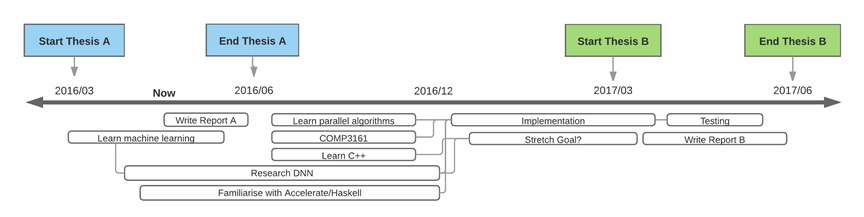
\includegraphics[width=\linewidth]{timeline.jpg}}
  \caption{Estimated timeline for this project.}
  \label{fig:timeline}
\end{figure}